% Capitolo 1

\chapter{Introduzione}

%    Il linguaggio adottato: Python ????
    
La conoscenza si colloca nella società come elemento fondamentale per un'economia avanzata. Il \emph{knowledge management} è una disciplina manageriale che si propone di studiarla e gestirla sotto gli aspetti culturali, organizzativi e tecnologici al fine di controllarla, diffonderla e replicarla.

Nella maggior parte dei casi le perle di saggezza emergono dalla conoscenza tacita, legata all'esperienza umana che risiede esclusivamente in ogni essere. L'\emph{expertise} rappresenta un vantaggio competitivo poiché permette, in pochi passi, di ottimizzare e migliorare processi.

L'acquisizione di nozioni derivate dall'esperienza è un notevole ostacolo per il knowledge management, motivo per cui l'ICT risulta essere un valido alleato per fornire i giusti strumenti atti alla gestione di tale sapere. In particolare, l'\emph{ingegneria della conoscenza} applica metodologie e formalismi per la progettazione di \emph{sistemi basati su conoscenza} allo scopo di acquisire, rappresentare, gestire, distribuire ed infine manutenere la conoscenza, con particolare attenzione e dedizione all'elaborazione dell'esperienza.

\begin{quotation}
\noindent \em You may have a Ph.D. in Computer Science, you may be a wiz programmer, but you couldn't do their job unless you underwent the right training and somehow acquired their troubleshooting experience\footnote{Introduction to Expert Systems (1998), cap. 1, pag. 1}.

\em Peter Jackson
\end{quotation}


La caratteristica fondamentale dei sistemi basati su conoscenza è quella di attuare una procedura d'\emph{inferenza} che, facendo uso della conoscenza codificata posseduta, renda possibile esibire un comportamento intelligente nel raggiungimento di un obiettivo in un determinato dominio di riferimento, utilizzando strategie di \emph{Problem Solving}. Tale intelligenza viene enfatizzata dal modo in cui tali sistemi si comportano in situazioni di incertezza e di parziale conoscenza del problema.

\section{Il problema della ricerca}
Un qualsiasi problema, per essere risolto, necessita di una o più soluzioni possibili se ne esistono. Pertanto, un generico problema può essere formulato nei seguenti termini:
\begin{itemize}
  \item Uno \textbf{stato di partenza}.
  \item Un \textbf{insieme di operazioni} che si possono applicare allo stato corrente per far evolvere (o regredire) un problema allo stato successivo (o precedente).
  \item Uno o più \textbf{stati finali} che rappresentano lo \textbf{spazio delle soluzioni} nonché gli obiettivi del problema se soddisfano un determinato \emph{test di terminazione}.
\end{itemize}

La rappresentazione dello spazio degli stati di un problema è un grafo connesso. Un semplice e primordiale algoritmo \emph{trial and error} potrebbe portare alla soluzione del problema. Tuttavia bisogna considerare due aspetti fondamentali nella ricerca di una soluzione:
\begin{itemize}
  \item Lo spazio di ricerca può essere finito ma ampio, oppure infinito.
  \item Il passaggio da uno stato all'altro potrebbe presentare la ripetizione di stati già visitati (loop).
\end{itemize}

Si possono adottare delle strategie alternative come la ricerca \emph{depth-first} e quella \emph{breadth-first}.

Entrambe le ricerche però potrebbero portare a computazioni decisamente complesse in spazi di ricerca molto grandi essendo esaustive. Inoltre, la depth-first search potrebbe raggiungere presto un obiettivo se fosse guidata da un qualche tipo di euristica ma potrebbe anche non terminare se lo spazio di ricerca fosse infinito, anche nel caso in cui vi sia una soluzione.

Si evince, quindi, che il numero di stati generati in ogni fase può crescere esponenzialmente, causando il cosiddetto fenomeno denominato \emph{esplosione combinatoria}. Per cui, tentare ad ogni step una ricerca per tutti i possibili stati di un problema corrisponderebbe ad un calcolo non indifferente equivalente a quello dato da un algoritmo di \emph{``brute force''}.

I problemi che richiedono un tempo che cresce esponenzialmente sono intrattabili e spesso rientrano nella classe dei problemi \emph{NP-completi}. Perciò, se un programma dovesse enumerare tutte le possibili mosse per il gioco degli scacchi, è evidente che non seguirebbe la strategia ideale per giocare una partita. Piuttosto, se un programma imitasse i grandi giocatori di scacchi, esibendo skill acquisite per selezionare strategie opportune e mosse vincenti, esso mostrerebbe un comportamento ``intelligente''.

Per ottenere una ricerca più efficiente, è stata introdotta la cosiddetta \textbf{ricerca euristica} o ricerca informata, che utilizza della conoscenza, tipicamente rappresentata da una funzione di valutazione che stima la distanza dall'obiettivo, per attraversare il grafo dello spazio degli stati del problema e, ad ogni passo, scegliere di procedere verso uno stato più vicino al goal da raggiungere.

Un'euristica può essere pensata come una regola empirica: a seconda dell'algoritmo o del processo di decisione scelto, il successo non è necessariamente garantito ma nella maggior parte dei casi la risoluzione del problema è facilitata. Sebbene la ricerca guidata da una funzione di valutazione euristica riduca notevolmente lo spazio di ricerca e permetta di trovare una soluzione migliore, talvolta questo approccio si rivela inadeguato per determinate applicazioni che richiederebbero comunque un tempo non ragionevole per giungere ad una soluzione (ad esempio nei task di pianificazione) oltre che costi elevati in termini di risorse.

Per affrontare le difficoltà di gestione della conoscenza descritte, si è cercato un approccio basato sull'utilizzo di regole di produzione, giungendo alla realizzazione di \emph{sistemi esperti}, capaci di rappresentare esplicitamente in dettaglio sia la conoscenza di un dominio posseduta da esperti, sia le strategie che essi utilizzano per ragionare sulla loro conoscenza (know-how).

I sistemi esperti fanno ampio uso della cosiddetta \textbf{programmazione euristica}, la quale, in contrapposizione alla programmazione algoritmica (che si basa su procedure matematicamente dimostrabili), permette di definire programmi che risolvono problemi senza un algoritmo definito a priori, determinando al momento, passo per passo, la sequenza di operazioni da eseguire.
 
\section{Rappresentare la conoscenza}

La rappresentazione della conoscenza è legata al processo attraverso il quale l'informazione può essere memorizzata ed associata nel cervello umano dal punto di vista della logica. Nell'ambito dei sistemi esperti, rappresentare la conoscenza significa descrivere in modo formale una mole consistente di informazioni affinché siano \emph{machine readable}. Descrivere formalmente l'informazione significa convertirla in un linguaggio non ambiguo che abbia una \emph{sintassi} ed una \emph{semantica}, allo scopo di governare forme di espressioni diverse, ciascuna con un significato ben definito. Quando la conoscenza è opportunamente codificata, può essere trattata con elaborazioni in cui simboli e strutture di simboli vengono utilizzate per rappresentare concetti e relazioni.
Un esempio per rappresentare in forma standardizzata la conoscenza è la situazione in cui si hanno frasi aventi sintassi diverse ma stesso significato:
\\

\hspace{1cm} \verb!Mario è il padre di Gianni.!\\

\hspace{1cm} \verb!Il padre di Gianni è Mario.!\\

\hspace{1cm} \verb!Gianni ha come padre Mario.!\\


Le frasi suddette hanno lo stesso significato, di conseguenza dovrebbero essere codificate in un unico modo. Un mapping in un'unica espressione per ogni frase potrebbe essere:
\\

\hspace{1cm} \verb!padre(Mario, Gianni).!\\

Come si può notare, il nome della funzione rappresenta la relazione (padre-figlio) che lega i due oggetti tra le parentesi, il primo oggetto è il padre ed il secondo il figlio. Questo linguaggio di rappresentazione è soltanto un esempio; esistono diversi formalismi per codificare la conoscenza. Il formalismo preso in considerazione per lo sviluppo di TURTLE è quello delle \emph{production rules} (regole di produzione) poiché costituisce un modello di calcolo molto diffuso nell'ambito dello sviluppo di sistemi esperti. Esso permette la rappresentazione dei più disparati domini, ha un forte potere espressivo per le euristiche, risulta essere molto flessibile nella definizione della notazione adottata per codificare l'esperienza e permette di \emph{guidare il ragionamento} tramite la codifica di strategie di controllo.

\section{Il modello computazionale}

\begin{quotation}
\noindent \em It is probably an axiom of artificial intelligence, and modern psychology, that intelligent behavior is rule-governed\footnote{Introduction to Expert Systems (1998), cap. 5, pag. 76}.

\em Peter Jackson
\end{quotation}


Le \emph{production rules} sono un formalismo utilizzato in diversi contesti tra cui i sistemi esperti (Buchanan and Feigenbaum, 1978). In questo ambito vengono spesso chiamate \emph{regole condizione-azione} perché codificano condizioni tra pattern di dati e azioni da eseguire nel caso in cui tali premesse siano soddisfatte.
\begin{figure}
  \center{CONDIZIONE $\xrightarrow{\hspace*{1cm}}$ AZIONE}
  \caption{Regola di produzione nella forma antecedente $\longrightarrow$ conseguente.}
\end{figure}

Le regole di produzione sono state introdotte da Post nel 1943 con la definizione di ciò che venne chiamato \emph{canonical system}, un sistema formale per la manipolazione di simboli. 
Un sistema a produzioni è composto dalle seguenti componenti:
\begin{itemize}
  \item Un \textbf{\emph{insieme di regole di produzione}} (altresì detto \emph{production memory}).
  \item Un \textbf{\emph{interprete di regole}} che decide quando e quali regole possono essere applicate.
  \item Un \textbf{\emph{database globale}} (o \emph{working memory}) che contiene la rappresentazione degli stati del problema, iniziali, intermedi ed obiettivo. Ogni elemento della working memory, di solito, prende il nome di \textbf{\emph{fatto}}. Una definizione più formale di cosa sia un fatto sarà illustrata a breve.
\end{itemize}

Nello scenario del funzionamento di un sistema a produzioni, la working memory viene esaminata e modificata dalle regole di produzione. Quest'ultime si attivano quando si verificano condizioni legate alla presenza di determinati fatti all'interno del database globale che soddisfino i pattern (dei fatti) presenti nella parte sinistra (LHS\footnote{Left hand side.}) di una o più regole. L'interprete delle regole ad ogni ciclo verifica quali di esse sono attivate e ne seleziona una. Questo ciclo macchina prende il nome di \textbf{recognize-act cycle}. Quando una regola è attivata, una o più azioni, presenti nella parte destra della regola (RHS \footnote{Right hand side.}), vengono eseguite. Le azioni possono apportare un cambiamento allo stato del problema consistente in modifiche ai fatti della working memory (aggiunte, aggiornamenti e rimozioni di fatti). Schematicamente, le regole in un sistema a produzioni sono nella forma:\\
\\
\indent $C_1, ..., C_m \rightarrow A_1, ..., A_n$\\
\\che si legge: \\
\indent se le \emph{condizioni} $C_1$ e ... e $C_m$ sono vere,\\
\indent allora esegui le azioni $A_1, ..., A_n$. \\

Come già accennato, l'\emph{interprete di regole} esegue delle operazioni non banali ad ogni ciclo \emph{recognize-act} (riconosci-agisci):
\begin{enumerate}
\item \textbf{\emph{Matching}}: consiste nella verifica delle condizioni nella parte sinistra di una regola, per ogni regola nell'insieme delle regole, rispetto ai fatti contenuti nella working memory. Al termine di questa verifica complessa, un sottoinsieme di regole attivabili viene restituito ed utilizzato nella fase successiva. 
\item \textbf{\emph{Risoluzione dei conflitti}}: se è possibile attivare più di una regola, allora un algoritmo (\emph{strategia di risoluzione dei conflitti}) seleziona la regola da applicare tra quelle presenti nel \emph{conflict set}. 
\item \textbf{\emph{Applicazione di una regola}}: eseguire le azioni nella parte destra della regola selezionata, quindi si ritorna al passo 1. Le azioni possono comprendere manipolazioni della working memory.
\end{enumerate}

La fase di \emph{matching} impone una notevole sequenza di controlli tra l'insieme delle regole ed il database globale essendo sostanzialmente un prodotto cartesiano tra due insiemi. Un esempio di matching semplice ma inefficiente, per una singola regola, sarebbe:\\

\indent \verb!Considera la regola! $r_i$\\
\indent \indent $\forall$ \verb!pattern! $p_j$ \verb!in! $r_i$\\
\indent \indent \indent $\forall$ \verb!fatto! $f_k$ \verb!nel db globale!\\
\indent \indent \indent \indent \verb!m! $\leftarrow$ \verb!match(!$f_k$\verb!,! $p_j$\verb!)!\\
\indent \indent \indent \indent \verb!se m è! $false$ \verb!allora restituisci! $false$\\
\indent \verb!restituisci! $true$\\

\begin{figure}
  \centering
  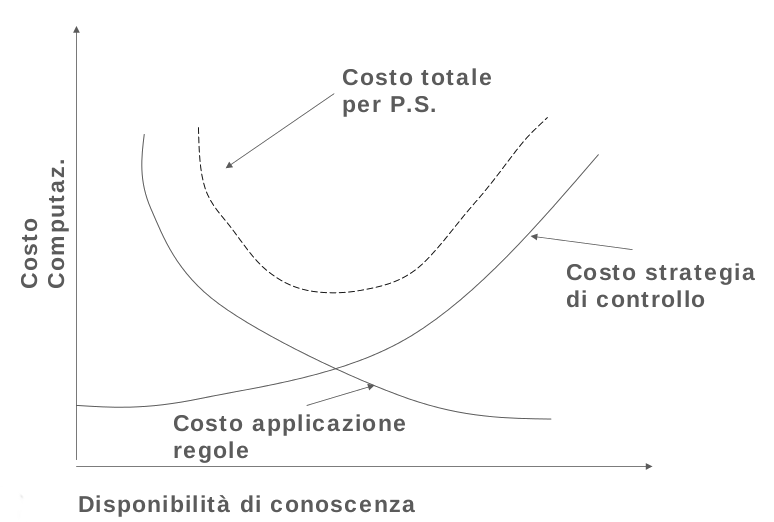
\includegraphics[scale=0.4]{pictures/costprod}
  \caption{Costo di un production system.}
  \label{fig:costo}
\end{figure}


Dall'esempio si evince che, all'aumentare della dimensione degli insiemi di fatti e regole il problema diventa intrattabile utilizzando scansioni lineari per ogni ciclo recognize-act. Inoltre, la funzione \verb!match! specificata esegue ulteriori controlli componente a componente per pattern, per cui si nota come il processo di \emph{matching} non sia banale.\\
Per quel che riguarda la risoluzione dei conflitti, è evidente che, se si definisse un insieme di regole, in cui, per ogni ciclo ne sia applicabile una ed una sola, allora si avrebbe un flusso deterministico paragonabile alla programmazione imperativa. Ciò che invece risulta essere tipico dei sistemi a regole è proprio il non-determinismo. Quest'ultimo è ancor più presente quando i pattern non sono composti solo da costanti ma anche da variabili. Tuttavia, affidarsi al totale non-determinismo è spesso controproducente in termini di efficienza nella ricerca di soluzioni per problemi di una certa consistenza (pur disponendo di un ottimo algoritmo di matching), motivo per cui, oltre alla risoluzione dei conflitti fornita di default da un interprete di regole, è possibile definire strategie di controllo del ragionamento attraverso \emph{meta-regole}, le quali modellano in modo più dettagliato relazioni ed oggetti di dominio. Da ciò si deduce che, una rappresentazione dettagliata e approfondita della conoscenza implica un costo più basso di attivazione delle regole. La figura ~\ref{fig:costo} esplica esaustivamente il concetto \footnotemark. 

\footnotetext{Principles of Artificial Intelligence (Nilsson, 1980).}

Nello sviluppo del sistema TURTLE si è considerato come software di riferimento il tool CLIPS (derivante dalla famiglia \verb!OPS5!)\footnote{C Language Production system - \url{http://clipsrules.sourceforge.net/}.}. Questo software fornisce diversi approcci per la rappresentazione della conoscenza per realizzare un sistema esperto. CLIPS è un sistema \emph{\textbf{forward chaining}} (concatenazione in avanti) in cui il match avviene tra le parti sinistre delle regole e la working memory mentre le azioni sono specificate nelle parti destre. Di conseguenza, anche TURTLE lavora concatenando in avanti. In contrapposizione al \emph{\textbf{backward chaining}}, che ha un approccio \emph{top-down}, il forward chaining è associato ad un approccio \emph{bottom-up}. Sebbene la concatenazione di simboli all'indietro sia indispensabile per problemi top-down (partendo da possibili goal), nulla vieta di risolvere il problema implementando il ragionamento all'indietro tramite forward chaining.

Essendo CLIPS un sistema molto vasto, in questo documento tratteremo solo le caratteristiche da cui si è attinto per realizzare TURTLE. Gli elementi fondamentali di entrambi i sistemi, ed in generale di tutti i sistemi a regole di produzione, sono i \textbf{fatti}, le \textbf{regole} ed il \textbf{meccanismo di matching}.
Per quel che concerne i fatti, la struttura del fatto preso in considerazione è l'\textbf{ordered fact} (fatto ordinato), definito formalmente come una ennupla $(\mu, \sigma_1, ..., \sigma_n)$, dove $\mu$ è il nome del fatto mentre ciascun $\sigma_i$ rappresenta un valore indicizzato per posizione.

\begin{figure}[here]
  \verb!    (padre Mario Gianni)!\\
  \verb!    (padre Antonio Nicola)!\\
  \caption{Una lista di fatti ordinati in CLIPS compatibile con TURTLE. Relazione padre-figlio.}
\end{figure}

\begin{figure}[here]
  \verb!    (defrule <nome-regola>!\\
  \verb!        (condizione_1)!\\
  \verb!        ...!\\
  \verb!        (condizione_m)!\\
  \verb!        =>!\\
  \verb!        (azione_1)!\\
  \verb!        ...!\\
  \verb!        (azione_n)!\\
  \verb!    )!
  \caption{Struttura della definizione di una regola in CLIPS compatibile con TURTLE. Si evince la sintassi LISP-like.}
\end{figure}


\section{I sistemi esperti}

Un sistema esperto è un programma, basato su conoscenza, che tenta di riprodurre il comportamento di un esperto umano in uno specifico dominio. In particolare fornisce le risposte o i consigli che fornirebbe l'esperto umano ed è in grado di giustificare la propria risposta.
I sistemi esperti consentono di risolvere problemi, la cui soluzione richiede una considerevole esperienza umana, ragionando euristicamente su una rappresentazione parziale della realtà del problema.

\begin{figure}[here]
  \centering
  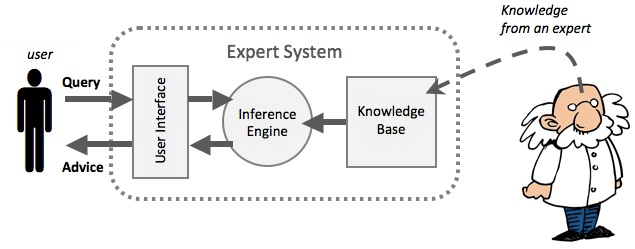
\includegraphics[scale=0.6]{pictures/expertsys}
  \caption{Come funziona un sistema esperto.}
  \label{fig:expertsys}
\end{figure}

Un sistema esperto è costituito da un'interfaccia, che ha il compito di rendere la comunicazione tra utente e sistema più naturale possibile, da una \emph{base di conoscenza}, che memorizza la conoscenza estratta dall'esperto (tale conoscenza consiste, essenzialmente, di fatti e di regole) e da un \emph{motore inferenziale}, parte attiva del sistema, che utilizza la base di conoscenza per inferire nuovi fatti e produrre soluzioni, ovvero simula il processo di ragionamento tramite il quale è possibile trarre delle deduzioni logiche partendo dall'esperienza presente nella base di conoscenza, ampliandola.

Un sistema esperto, inoltre, incapsula un modulo per la spiegazione della soluzione che \emph{\textbf{fornisce indicazioni sulle modalità di ragionamento}} e di \emph{\textbf{giustificazione delle scelte intraprese}} per giungere ad una soluzione.

